\end{multicols*}
\begin{center}
\mysection{Kismet}{adventurer-kismet}

\summary {
    \begin{center}
    
    Your Adventurer's \mybold{Kismet} represents the intervention of the Fates in their lives. Kismet has three aspects: Death, Injury, and Insanity.

    \myskip

    Each aspect of your Adventurer's Kismet starts at a d3.
    \end{center}
}
\end{center}

\mylist {

    \item  \DEATH\: \mybold{Death:} try your Death die once (or more!) at the \mybold{Top of the Moment} whenever you are at 0 Flesh. More details can be found in the section on \mypg{Dying}{combat-dying}.
    \item  \INJURY\:  \mybold{Injury:}  try your Injury die when you survive \mybold{Dying}, or at the Arbiter's discretion if something particularly heinous happens to you.
    \item  \INSANITY\: \mybold{Insanity:} try your Insanity die whenever you experience something terrifying or horrifying at the Arbiter's discretion.
}

  \myimage{adventurer/Skull1}


\newpage

\begin{center}
\mysubsection{Death}{adventurer-kismet-death}
\summary {
\begin{center}
   Your \DEATH starts at \mybold{Precarious (d3)}.
\end{center}
}
\end{center}
\begin{multicols*}{2}\raggedcolumns


  \myimage{adventurer/CloakDeath}

\cbreak

If your Flesh ever goes to 0, you are \mypg{Dying}{combat-dying}. While your Flesh is at 0 you will need to try a \RS with your Death die at the Top of each Moment.

If you roll a Failure, you immediately perish!

Unless noted in your Trope or Species, your Death die starts at Precarious (d3).  You can improve your Death die during \mypg{Advancement}{advancement}.

  \mytable{X c}{
    \thead{} & \thead{\DEATH} \\
  }{
      Precarious & d3 \\
      Tough & d4  \\
      Resilient & d6 \\
      Enduring & d8 \\
      Amaranthine & d10 \\
  }


\newpage
\end{multicols*}



\mysubsection{Injury}{adventurer-kismet-injury}

\flavor{"I suppose nothing hurts you."  

"... Only pain" \\~ \Tilde \mybold{Conan the Destroyer}}


  \myctrtable{Y Y}{
    \thead{} & \thead{\INJURY} \\
  }{
      Fragile & d3 \\
      Solid & d4  \\
      Durable & d6 \\
      Unbreakable & d8 \\
      Adamantine & d10 \\
  }

\summary {
   \begin{center}
   Your \INJURY starts at \mybold{Fragile (d3)}.
    \end{center}
}


Adventuring is dangerous business, and it's not uncommon for Adventurers to receive permanent physical injury. If you survive Dying, or if something particularly heinous happens to you (a fall from a great height, thrown by a Giant, etc.) you must try your \INJURY die. If you roll a Failure on an Injury try, roll a d10 on the table below to see what happens.

Unless an Injury is \mybold{Permanent}, you can have it healed through the ministrations of a medic. Injuries can only be healed in a \mypg{Settlement}{civilization-settlements}. If someone in your Band knows the \mypg{Vulgate of Medicine}{vulgate-medicine}, they can heal your injuries; otherwise you must engage the services of a \mypg{Chirugeon}{gear-services}.

\myhighlight{Wound}{physical-wound}

  \mytable{c X}{
    \thead{d10} & \thead{} \\
  }{
      1 & Superficial dueling scar. You say where it is. \mybold{Permanent} \\
      2 & Knocked out d3 teeth. You say which ones. No effect if you're wearing a \mypg{Helmet}{gear-armor} (unless you want to lose the teeth). Roll again if you're out of teeth. \mybold{Permanent} \\
      3 & Badly broken nose; even when it's fixed you'll have difficulty smelling and tasting things from now on. No effect if you're wearing a Helmet (unless you want a broken nose). If you've already had this Injury, roll again.  \mybold{Permanent} \\
      4 & Lose a finger or toe - your choice \mybold{Permanent} \\
      5 & Broken hand. You can't do anything requiring fine motor coordination (does not include \mypg{Arcana}{arcana} or \mypg{Whispers}{vulgate-whispers}). \\
      6 & Pulled a shoulder muscle. Brawl and Throw weapons deal -2 to any damage (minimum 1). \\
      7 &  Got your bell rung. No effect if you were wearing a Helmet. You can't do anything requiring \mybold{Concentration}. \\
      8 &  Twisted your knee or ankle.  Shift your \MD \DCDOWN. \\
      9 &  Feeling your age.  You are unable to heal Grit. \\
      10 & Serious injury. Roll on the \mybold{Beating} table instead. \\
}

\newpage


\myhighlight{Beating}{physical-wound-beating}

  \mytable{c X}{
    \thead{d10} & \thead{} \\
  }{
      1 & You've injured your (1-3 left, 4-6 right) 1) Hand; 2) Forearm; 3) Elbow; 4) Bicep; 5) Triceps; 6) Underarm.  Whichever arm got hit is useless - you can't hold anything with it. You can't use 2h weapons. If you try to fight with your "off hand", your Attack \RO checks are at -4 and you deal -2 damage (minimum 1).  If you don't know which one is your "main" hand, roll a d6: 1-4 it's your right, 5-6 it's your left. \\
      2 & You've injured your (1-3 left, 4-6 right)  1) Foot; 2) Shin; 3) Calf; 4) Knee; 5) Thigh; 6) Hip  You can't run and can only walk with a limp.  Your \MD drops \DCDOWN x2 (meaning you're immobile if you're wearing heavy armor). \\
      3 & You've injured your 1) Cheek; 2) Ear; 3) Mouth; 4) Nose; 5) Jaw; 6) Eye.  That's pretty rough to look at.  If you're wearing a Helmet, no effect but the helmet is destroyed.  Until you receive medical care, people will find you grotesque and repugnant. The injury leave you permanently disfigured.  Make an immediate \INSANITY try. \\
      4 & Right in the goods. Everyone winces, you drop to the fetal position for Minutes and can't move, even to defend yourself.  Kids are probably out of the question.  You can't heal any Grit until the Wound is taken care of. \\
      5 & Injury to your 1) left upper; 2) right upper; 3) left lower; 4) right lower back!  Immediately set your \mypg{Burden}{gear-burden} to 0 i.e. you can't carry any significant items (including armor and weapons). \\
      6 & Your 1) throat; 2) back of neck; 3) left side of neck; 4) right side of neck; 5) left shoulder; 6) right shoulder is hurt. If it's your shoulder, same as "Arm" above.  If it's your throat or neck, you are unable to speak, meaning you can't use any Arcana or Vulgates that require speech. \\
      7 &  Your (1-3 left, 4-6 right) chest and ribcage are injured. Any time you do anything strenuous (like Attacking, Guarding, or running away), make a \RSTRY{\VIG} try. If you Fail, you are inflicted with \effect{the Vapors}. \\
      8 &  Abdominal wound. You stuff your intestine back inside your body.  Any time you do anything strenuous (like Attacking, Guarding, or running away), make a \RSTRY{\VIG} try. If you Fail, you are inflicted with \effect{Bleeding}. \\
      9 &  Blow to the spine. You're partially paralyzed and can only crawl. You are inflicted with \effect{Prone} until you can receive medical attention in a \mypg{Settlement}{civilization-settlements}. \\
      10 & You take it to the cabbage. Helmets save lives - if you were wearing a Helmet, it's destroyed but you're otherwise OK.  Otherwise you immediately fall comatose: 
treat as having a permanent infliction of \effect{the Vapors} until you can receive medical attention in a \mybold{Settlement}. \\
}


\begin{center}
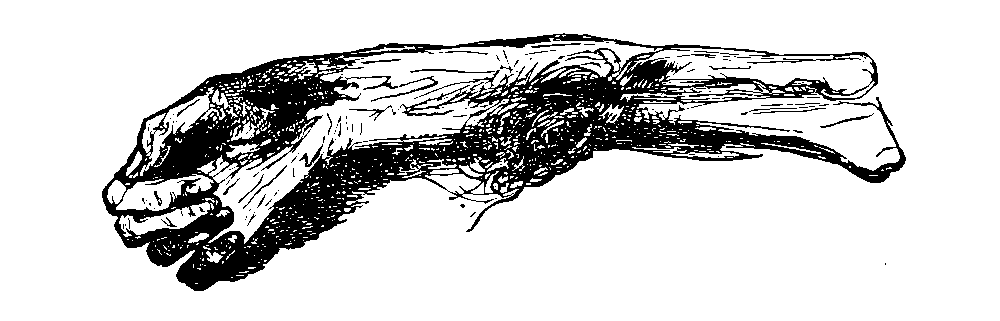
\includegraphics{adventurer/KismetArm}
\end{center}



\newpage

\mysubsection{Insanity}{adventurer-kismet-insanity}


  \myctrtable{Y Y}{
    \thead{} & \thead{\INSANITY} \\
  }{
      Pliant & d3 \\
      Sober & d4  \\
      Rational & d6 \\
      Abiding & d8 \\
      Unwavering & d10 \\
  }

\summary {
   \begin{center}
   Your \INSANITY starts at \mybold{Pliant (d3)}.
    \end{center}
}



The Arbiter can ask for an Insanity try at any time if they warrant something extremely disturbing has happened. For example:  witnessing a member of the Band getting killed; encountering some horrifying creature you've never seen before; or surviving a brush with \mypg{Death}{combat-dying}. If you roll a Failure on an Insanity try, roll a d10 on the table below.

Unless an Insanity is \mybold{Permanent}, you can be rehabilitated through a dose of \mypg{Laudanum}{research-chymistry-laudanum}; through the miracle of \mypg{Sin Eating}{miracle-sin-eating}; or by the services of a \mypg{Chirugeon}{gear-services} in a \mybold{Settlement}. 


  \mytable{l X}{
    \thead{d10} & \thead{} \\
  }{
      1 & Develop a nervous tic. You say what it is. \mybold{Permanent} \\
      2 & You often find yourself muttering under your breath. If you already have this Insanity, roll again. \mybold{Permanent} \\
      3 & Your hair turns snow white. If you already have this Insanity, roll again. \mybold{Permanent} \\
      4 &  Partial Amnesia. Your Adventurer will not remember what happened from the beginning of the Session up to this point. \mybold{Permanent} \\
      5 &  Hysterical Blindness.  You can only see things Close or Nearby and thus can't use Shoot weapons. \\
      6 &  Distracted.  You can't do anything requiring \mybold{Concentration}. \\
      7 &  The Shakes. You can't do anything requiring fine motor coordination (does not include \mypg{Arcana}{arcana} or \mypg{Whispers}{vulgate-whispers}). \\
      8 &  Gullible. Sleep and Charm Person work on you automatically, and you'll tend to believe anything someone says. \\
      9 &  Rattled.  You are unable to heal Grit. \\
      10 &  Your mind breaks. Roll on the \mybold{Madness!} table instead. \\
}

\newpage

\myfpimage{adventurer/InsanityDetail}

\myhighlight{Madness!}{injury-insanity-madness}

  \mytable{c X}{
    \thead{d10} & \thead{} \\
  }{
        1 & \mybold{Darkfear} You are terrified of the dark. You cannot sleep in darkness; you must have a burning candle or lamp by your side or you do not gain any of the benefits associated with a Bivouac. When you are in pitch darkness you are utterly helpless - you automatically fail any \RO or \RB tries. \\
        2 & \mybold{Foolhardiness} Your continued survival in the face of the unnatural has given you the irrational belief that you are invincible. You cannot retreat or withdraw from dangerous situations unless you are unconscious (or dead).\\
       3 & \mybold{Gluttony} You are overcome by the irrational belief that if you consume you will not be consumed by your fear. You refuse to wear armor since it's "binding".  If you Bivouac, roll your Personal Provisions 3 times.  Your extra weight counts as 2 \mypg{Burden}{gear-burden}.\\
        4 & \mybold{Melancholy} You are consumed by depression and ennui. Before you make any \RO or \RB try, you must \RS{\FOC}. If you roll a Failure, you refuse to take the \RO or \RB try (if you are in Combat, the feeling goes away after a Moment).\\
        5 & \mybold{The Needle} Only \mypg{Drugs}{gear-narcotics} will stave off the gnawing terror. Roll a d12 on the \mypg{Narcotics}{gear-narcotics} table - you are \mybold{Addicted} to that substance. If it's not immediately available to you, you are inflicted with \effect{Sickened}.\\
       6 & \mybold{Night Terrors} You are unable to Bivouac unless you first try \INSANITY. Failure means you cannot rest, in addition to the effect of the \INSANITY try.\\
       7 & \mybold{Overwhelmed} Your madness has left you periodically deaf and dumb to the world around you as you retreat within yourself to escape your fear. Your \mypg{Grit}{adventurer-flesh-grit} is 0 while under the effects of this madness and can't be healed, and you always lose Init.\\
       8 & \mybold{Shot Nerves} Your madness has weakened your already fragile mental state.  Whenever you enter Combat or a stressful situation (determined by the Arbiter), roll a \RSTRY{\INT}.  If you fail you can only stand gawping in horror for the rest of Combat.  You cannot Attack or Guard, but you can be pulled / moved by Allies.\\
       9 & \mybold{Starvation} Your madness has inspired the irrational belief that if you deny yourself food you can deny the extent of your fear. Whenever you Bivouac, roll a \RSTRY{\FOC}  If you fail you are unable to consume your Personal Provisions (and thus get no benefit for resting).  You are unable to heal Grit.\\
      10 & \mybold{The Voices} You are continually distracted by a number of voices that only you can hear. Each time you roll Init, make an \RSTRY{\FOC}  If you fail you are inflicted with \effect{Befuddled} for the rest of Combat. You fail all \mypg{Listen}{skill-listen} skill rolls.\\

}


\newpage
\begin{multicols*}{2}\raggedcolumns
